\documentclass[t]{beamer}
\usepackage{listings}
\usepackage{minted}

\usetheme{default}
\usebackgroundtemplate{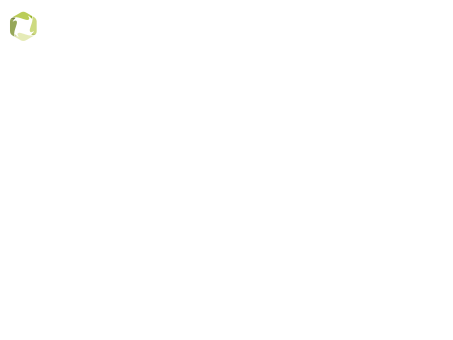
\includegraphics[width=\paperwidth]
                                       {../cpeb_bkground_topleftlogo.pdf}}

\setbeamertemplate{frametitle}{
  \centering\vspace{1mm}\insertframetitle\par\vspace{3mm}
}

\usepackage[style=nature,
            hyperref,
            backend=biber,
            isbn=false,
            doi=false,
            url=false,
            date=year,
            maxbibnames=3
           ]{biblatex}

\bibliography{kdm-apr.bib}

\title{Novel algorithms for population-scale analysis of plant genomes}
\subtitle{\small{Annual Plan Review}}
\author{Kevin Murray}
\institute{Borevitz Lab, CPEB, ANU}
\date{24 July 2015}

\begin{document}

{
\usebackgroundtemplate{
\includegraphics[width=\paperwidth]{../cpeb_bkground_centered.pdf}}
\begin{frame}
  \titlepage
  \vfill
\end{frame}
}


\begin{frame}{Understanding Plant Function and Variation}
  \begin{itemize}
    \item We want to understand function of plant systems
    \item Genetic variation in these systems important
  \end{itemize}
  \begin{center}
    \includegraphics[width=0.6\textwidth]{img/rice-paddy.jpg}
  \end{center}
  \tiny{\url{irri.org}}
\end{frame}


\begin{frame}{Existing genetic approaches}
  \begin{itemize}
    \item Forward genetics
      \begin{itemize}
        \item Select trait/phenotype
        \item Randomly mutate genome
        \item Screen, map loci affecting phenotype
        \item (read backwards is reverse genetics)
      \end{itemize}
    \item Association mapping in populations
      \begin{itemize}
        \item Select parents by phenotype, cross
        \item Examine variation in phenotype across population
        \item Associate phenotype with genotype, map loci
      \end{itemize}
    \pause
  \item These approaches \textbf{diversity limited}: ``missing heritability''
  \end{itemize}
\end{frame}


\begin{frame}{Missing heritability in the field?}
  \begin{itemize}
    \item Find more diversity in the field!
    \item Sample natural populations
      \begin{itemize}
        \item Ecological hypotheses of trait selection, adaptation
        \item Sample widely as possible across non-uniform genetic diversity
      \end{itemize}
      \pause
    \item Now \textbf{complexity limited}: complex kinship \& population
      structure
    \item Mandates development of economic, accurate large scale population
      genomics
  \end{itemize}
  \begin{center}
    \includegraphics[width=\textwidth]{img/jared-tree.pdf}
  \end{center}
\end{frame}

\begin{frame}{Large-scale genome analysis}
  \begin{itemize}
    \item Moving from 100s to 1000s and 10000s of samples \textit{per PhD!}
      \pause
    \item Efficient algorithms to analyse large-scale genomic data
    \begin{itemize}
      \item Reference \& alignment free: \textit{less bias, de novo}
      \item Platform/protocol agnostic: \textit{future proof}
      \item Computationally efficient: \textit{not the bottleneck}
      \item Cross scale: \textit{one tool to rule them all}
    \end{itemize}
  \end{itemize}
  \begin{center}
    \includegraphics[width=\textwidth]{img/cross-scale.png}
  \end{center}
  \tiny{after \textcite{peterson_double_2012}}
\end{frame}


\begin{frame}{$k$-mer analysis}
  \begin{columns}[t]
    \column{0.6\textwidth}
      \begin{itemize}
        \item<1-> Analyse $k$-length words of sequences
        \item<2> Computationally and biologically appropriate
        \begin{itemize}
          \item<2> Fast
          \item<2> Constant-memory (using \texttt{khmer})
          \item<2> Scalable and parallelisable
          \item<2> Cross-scale
        \end{itemize}
      \end{itemize}
      \vfill
    \column{0.4\textwidth}
    $k = 3$\\
    \texttt{ACGTGT}\\
    \texttt{ACG~~~}\\
    \texttt{~CGT~~}\\
    \texttt{~~GTG~}\\
    \texttt{~~~TGT}
  \end{columns}
\end{frame}

\begin{frame}{Thesis overview}
  \begin{itemize}
    \item \textit{in silico}, experiment-driven software development
      \begin{itemize}
        \item New tools, and new combinations of tools (pipelines)
        \item Multi-layered analysis of large population sequencing projects
      \end{itemize}
    \pause
    \item Chapter 1: $k$-mer based clustering of next gen sequencing
      \begin{itemize}
        \item First-pass basic clustering
        \item \textit{kinship/relatedness}
      \end{itemize}
    \pause
    \item Chapter 2: Machine learning for population genomics
      \begin{itemize}
        \item Detailed analysis of $k$-mer genetic distance
        \item \textit{population structure, visualisation, sample classification}
      \end{itemize}
    \pause
    \item Chapter 3: Population ``genome-typing by sequencing''
      \begin{itemize}
        \item Pan-genome variant calling
        \item \textit{genome-wide genotyping through whole genome sequencing}
      \end{itemize}
  \end{itemize}
\end{frame}

\begin{frame}{$k$-mer based clustering}
  \begin{itemize}
    \item Extend alignment-free sequence comparison to raw NGS data
    \item Have released new software package: \texttt{kWIP}
      \begin{center}
        \includegraphics[width=0.9\textwidth]{img/kwip-doc-screenshot.png}
      \end{center}
  \end{itemize}
\end{frame}

\begin{frame}{\texttt{kWIP}}
  \begin{itemize}
    \item The $k$-mer Weighted Inner Product
    \pause
    \item Algorithm:
      \begin{itemize}
        \item For each sample: count all $k$-mers into a Count-Min Sketch
        \pause
        \item For each analysis set, i.e ``population'':
          \begin{itemize}
            \item Calculate the informational entropy of CMS bins ($H$)
            \item For each pair of samples $A$ and $B$, calculate
              $\sum^{n}_{i=0} A_i \cdot B_i \cdot H_i$
          \end{itemize}
      \end{itemize}
    \pause
    \item The software:
      \begin{itemize}
        \item \texttt{C++}, $>$2000 lines of code
        \item Uses \texttt{khmer} for $k$-mer counting \& hashing
        \item Parallelised, $\approx$ 10 hrs for 96 rice samples.
        \item GNU GPL licensed, source code released on GitHub
      \end{itemize}
    \item Paper in Prep
  \end{itemize}
\end{frame}


\begin{frame}{\texttt{kWIP} Experiments}
  \begin{itemize}
    \item 3000 rice genomes:
      \begin{itemize}
        \item 3000 rice lines from known families
        \item Analysing in sets of $\approx 200$, from all major groups
        \item Recover known grouping w/ \texttt{kWIP}, not w/ unweighted IP
        \item Sensitive to read depth
      \end{itemize}
    \item Simulation
      \begin{itemize}
        \item Fake population genome sequencing studies
        \item Experiments in progress, early results positive
        \item Test limitations of \texttt{kwip}
      \end{itemize}
    \item Protocol optimisation
      \begin{itemize}
        \item Effect of varying $k$
        \item Effect of CMS size
        \item More appropriate normalisation
      \end{itemize}
  \end{itemize}
\end{frame}


\begin{frame}{Machine learning for Population Genomics}
  \begin{itemize}
    \item How to maximise amount of information $k$-mer abundance provides?
      \begin{itemize}
        \item Pairwise genetic distance: \texttt{kWIP}
        \item Admixture
        \item Online clustering (not all pairs)
        \item Visualisation of distance and confidence
      \end{itemize}
      \pause
    \item Experiments
      \begin{itemize}
        \item Detect known introgression and admixture in 3000 rice lines
          dataset
        \item Investigate on-line classifier for novel rice samples: ``who am I''
        \item Develop HTML5 visualisation of \texttt{kWIP} output
      \end{itemize}
  \end{itemize}
\end{frame}


\begin{frame}{Progress}
  \begin{itemize}
    \item First-pass basic clustering
      \begin{itemize}
        \item \texttt{kWIP} implemented \& optimised
        \item Experiments in progress, some complete
        \item Paper in prep
      \end{itemize}
      \pause
    \item Machine Learning
      \begin{itemize}
        \item Collaborations started
        \item Initial experiments planned
      \end{itemize}
      \pause
    \item Population pan-genome variant calling: \textit{``genome-typing by sequencing''}
        \begin{itemize}
          \item Initial collaborations started (DIB-lab)
          \item Evaluating published tools
        \end{itemize}
  \end{itemize}
\end{frame}

\begin{frame}{Thanks}
  \begin{itemize}
    \item Justin, Norman, Sylvain, Gavin and Barry
    \item Cheng Soon Ong, Christfried Webers
    \item C. Titus Brown, Michael Crusoe, Camille Scott (DIB-lab) @ UC Davis
    \item Kenneth McNally/IRRI
    \item Yourselves
  \end{itemize}
\end{frame}

\begin{frame}[shrink=20]{References}
  \printbibliography
  \vfill
  .
\end{frame}

\begin{frame}{Side Projects}
  \begin{itemize}
    \item Reduced Representation Sequence Filtering
      \begin{itemize}
        \item de Bruijn graph based filter/normaliser
        \item With GDU/ABC
      \end{itemize}
    \item $k$-mer approaches to detect horizontal gene transfer
      \begin{itemize}
        \item Collaboration with Adam Taranto
      \end{itemize}
  \end{itemize}
\end{frame}


\begin{frame}{\texttt{kWIP} Distance Matrices}
  \begin{center}
    \includegraphics[width=\textwidth]{img/weight-unweight.png}
  \end{center}
\end{frame}

\begin{frame}{Population Re-structuring}
  \begin{center}
    \includegraphics<1>[width=\textwidth]{img/restruct-1}
    \includegraphics<2>[width=\textwidth]{img/restruct-2}
    \includegraphics<3>[width=\textwidth]{img/restruct-3}
  \end{center}

  \tiny{after \textcite{brachi_genome-wide_2011}}
\end{frame}

\end{document}
